\section{Durchführung}
\label{sec:Durchführung}

Der Versuchsaufbau ist schematisch in Abbildung \ref{fig:aufbau} zu sehen. Er besteht aus einer Lichtquelle, deren Licht durch einen Kondensator auf einen 
Lichtmodulator fällt. Dieser kann durch ein Steuerungselement auf eine beliebige Frequenz eingestellt werden. Hinter dem Modulator befindet 
sich ein Glan-Thompson-Prisma, welches mit einem Ganiometer verbunden ist und sich durch eine Drehung an letzterem als Polarisator verwenden 
lässt. Die Funktionsweise eines solchen Prismas ist in Abbildung \ref{fig:prisma} dargestellt.

\begin{figure}
    \centering
    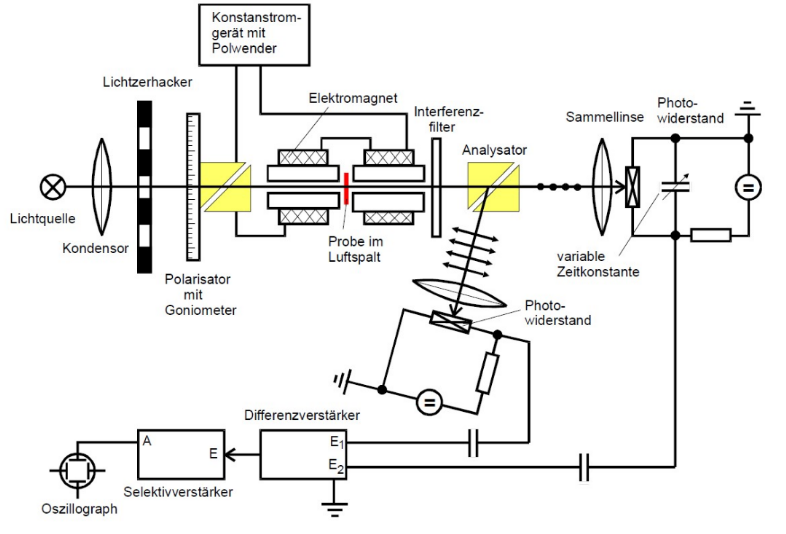
\includegraphics[scale=0.3]{content/Aufbau.png}
    \caption{Schematischer Aufbau des Versuchs \cite{anleitung}.}
    \label{fig:aufbau}
\end{figure}

\begin{figure}
    \centering
    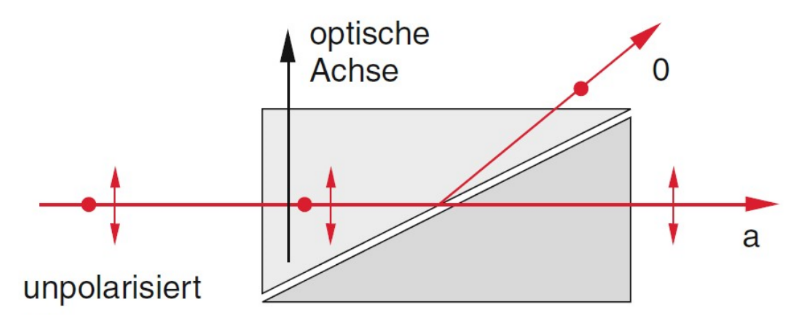
\includegraphics[scale=0.3]{content/prisma.png}
    \caption{Schematischer Aufbau eines Glan-Thompson Prismas \cite{anleitung}.}
    \label{fig:prisma}
\end{figure}

Das austretende Licht fällt durch einen Elektromagneten, in dessen Mitte sich ein Luftspalt befindet, in dem die Probe eingelassen werden kann. 
Bei Austreten des Strahls fällt das Licht auf einem Interferenzfilter, der es ermöglicht Licht nur einer Wellenlänge zu betrachten. Dieses Licht
wird wiederum an einem zweiten Glan-Thompson-Prisma in zwei Strahlenbündel geteilt, die dann auf Photodetektoren treffen. Die so entstehenden 
Signale der beiden Detektoren werden auf die Eingänge eines Differenzverstärkers gegeben, dessen Ausgangsspannung proportional zur Differenz 
der beiden Signale ist. Das Signal wird dann auf einen Selektivverstärker gegeben, der auf die gleiche Frequenz wie der Lichtmodulator gestellt 
wird. Dies ermöglicht eine Unterdrückung des auftretenden Hintergrundrauschens, wenn die Güte des Verstärkers $Q = 100$ beträgt. Das Ausgangssignal
kann dann an einem Oszillograph dargestellt werden. \\

Bevor der eigentliche Versuch beginnen kann muss der Aufbau justiert werden. Dazu wird zunächst ein freier Stahlengang betrachtet. Die Halogenlampe 
wird auf $\SI{10}{\volt}$ eingestellt. Dann werden die Prismen so gedreht, dass die Strahlenbündel möglichst senkrecht auf die Prismen fallen. Das 
Licht soll dann so auf die Detektoren treffen, dass bei geeigneter Drehung des Polarisationsprimsas die Lichtintensität an einem der Detektoren 
verschwindet und beim anderen maximal wird. Dann wird für den Lichtmodulator sowie den Selektivverstärker eine Frequenz von $\SI{450}{\hertz}$
eingestellt. Dann wird der Elektromagnet auf $\SI{10}{\ampere}$ hochgefahren und eine der Proben sowie ein Interferenzfilter eingesetzt. Die Photodetektoren
werden nun mit der Verstärkerelektronik gemäßg Abbildung \ref{fig:aufbau} verbunden. Anschließend wird durch Drehen des Polarisationsprimsas 
geprüft, dass die Signalamplitude am Oszillograph unter einer Periodizität von $\SI{90}{\degree}$ minimal wird. \\

Nach der Justierung kann mit der eigentlichen Messung begonnen werden. Dazu werden zwei n-dotierte und eine hochreine GaAs-Probe zu jedem der 
neun verschiedenen Interferenzfilter vermessen. Dabei wird dann zu jeder der neun Wellenlängen ein Winkel am Ganiometer abgelesen und notiert, 
unter dem die Signalamplitude minimal wird. Das Magnetfeld wird nach jeder Messung umgepolt und die Messung wiederholt. Aus der Differenz der 
beiden gemessenen Winkel lässt sich dann die Faraday Rotation $\theta = \theta_1 - \theta_2$ berechnen. Nach der Messung der drei Proben 
wird das Magnetfeld zur Bestimmung der maximalen Kraftflussdichte $B_\text{max}$ an der Stelle der Probenhalterung mit einer Hallsonde vermessen.
